\documentclass[tikz, border=0pt]{standalone}
\usepackage{tikz}
\usetikzlibrary{calc}

\begin{document}
\begin{tikzpicture}

% ── Colours ──────────────────────────────────────────────────
\definecolor{orbbec}{HTML}{00838A}
\definecolor{realsense}{HTML}{1565C0}
\definecolor{battery}{HTML}{EF6C00}
\definecolor{jetson}{HTML}{2E7D32}

% ── Block style (matches FSM state style) ────────────────────
\tikzset{
  block/.style={
    rectangle,
    rounded corners=3pt,
    draw=#1!70,
    fill=#1!30,
    thick,
    font=\footnotesize,
    align=center,
    minimum width=2.2cm,
    minimum height=1.0cm,
    inner sep=6pt,
  }
}

% ── CAD image (centre) ───────────────────────────────────────
% Replace fusion360_assembly.png with the real Fusion 360 render.
\node[inner sep=0] (cad) {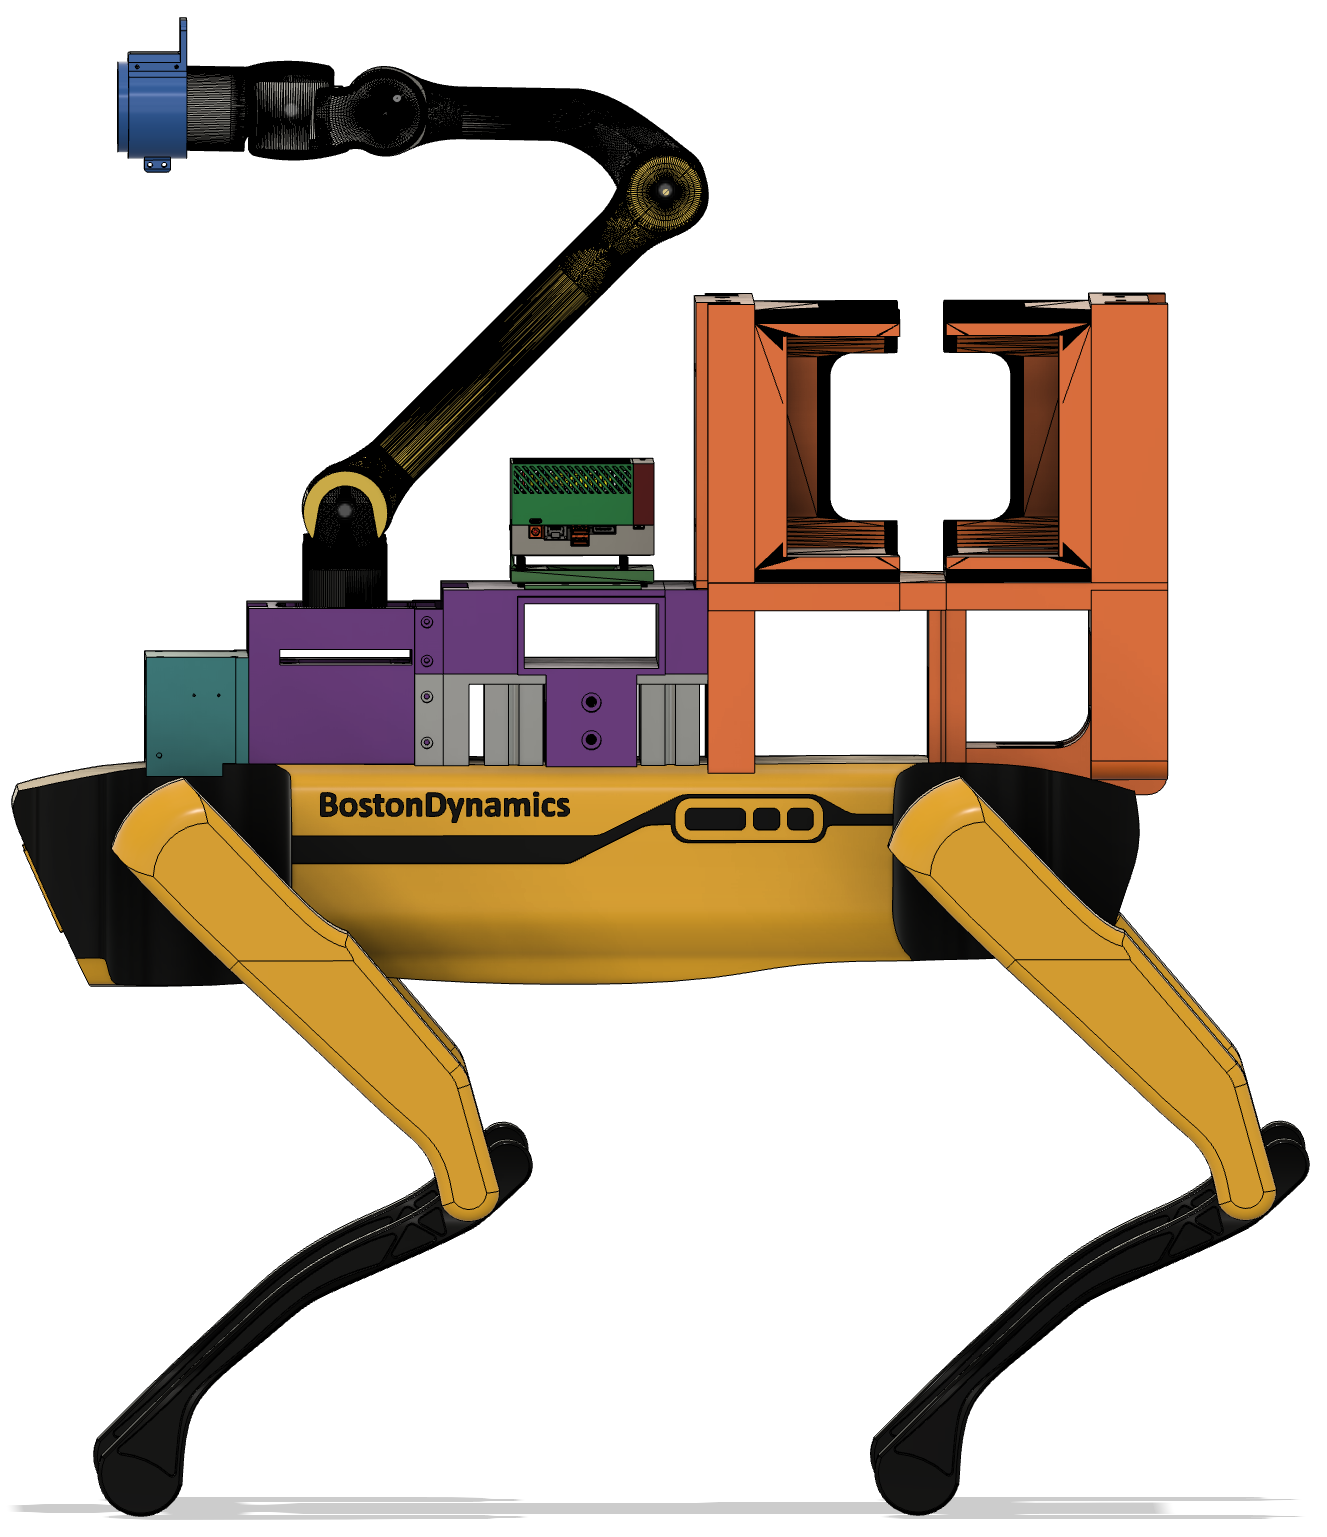
\includegraphics[width=5.2cm]{fusion_overview.png}};

% ── Vertical anchors ─────────────────────────────────────────
\coordinate (topL) at ($(cad.north west)!0.25!(cad.south west)$);
\coordinate (botL) at ($(cad.north west)!0.75!(cad.south west)$);
\coordinate (topR) at ($(cad.north east)!0.25!(cad.south east)$);
\coordinate (botR) at ($(cad.north east)!0.75!(cad.south east)$);

% ── Left blocks ──────────────────────────────────────────────
\node[block=realsense]
      at ([xshift=-1.3cm]topL) {Intel RealSense\\D415 mount};

\node[block=orbbec]
      at ([xshift=-1.3cm]botL) {Orbbec Femto\\Bolt case};

% ── Right blocks ─────────────────────────────────────────────
\node[block=battery]
      at ([xshift=1.3cm]topR) {Auxiliary\\Battery case};

\node[block=jetson]
      at ([xshift=1.3cm]botR) {Jetson Orin\\AGX holder};

\end{tikzpicture}
\end{document}
